\documentclass[10pt]{book}
\usepackage{graphicx}
\usepackage{subfig} % make it possible to include more than one captioned figure/table in a single float
\usepackage[utf8]{inputenc}
\usepackage{hyperref}
\usepackage[intlimits]{amsmath}
\usepackage{amssymb}
\usepackage{tkz-euclide}
\usepackage{tikz}
\setlength{\oddsidemargin}{15.5pt} 
\setlength{\evensidemargin}{15.5pt}
\pretolerance=2000
\tolerance=3000
\renewcommand{\figurename}{Figura}
\renewcommand{\chaptername}{Cap\'{i}tulo}
\renewcommand{\contentsname}{\'{I}ndice}
\renewcommand{\tablename}{Tabla}
\renewcommand{\bibname}{Bibliograf\'{i}a}
\renewcommand{\appendixname}{Ap\'endices}


\usepackage{geometry}
 \geometry{
 a4paper,
 left=15mm,
 right=10mm,
 top=20mm,
 bottom=20mm,
 }

\begin{document}
\paragraph 1 
\textbf{Notaciones}:
\begin{description}
	\item para p scalar notamos $\vec{\nabla} p = (\frac{\partial p}{\partial x_i})_{i=1,2,3}$	que es un vector
	\item para el vector $\vec{f}$ notamos $\nabla \vec{f}  = \sum_{i=1}^3 \frac{\partial f_i}{\partial x_i}$ que es un scalar	
	\item $\nabla^2 = \nabla \vec{\nabla}$	
\end{description}



\textbf{Ondas acústicas}:
En estado de equilbrio con las variables $p_0$, $\rho_0$ (constantes porque el medio es homogéneo) y  $\vec{v_0}$=0  
producimos perturbaciones $p_1$, $\rho_1$, $\vec{v}$ y las variables devienen:

$p = p_0 + p_1$

$\rho = \rho_0 + \rho_1$

$\vec{v}$

Las perturbaciones $p_1$, $\rho_1$, $\vec{v}$ son pequeñas de tal  forma que podemos despreciar los términos de  orden $\ge 2$ en las ecuaciones de conservación de masa y momento que  se pueden escribir:

ecuación de conservación de masa: $\frac{\partial \rho_1}{\partial t} + \rho_0 \nabla \vec{v}  = 0$ (1)

ecuación de conservación de momento: $\rho_0 \frac{\partial \vec{v}}{\partial t} = -\vec{\nabla} p_1$ (2)

ecuación de gas ideal: $p = \rho \frac{k_B}{m} T$

Las oscilaciones se producen a temperatura constante $\implies p = c_s^2 \rho $ donde notamos la constante $c_s= \sqrt{\frac{k_B}{m} T}$ (velocidad de sonido en condiciones isotermas )

(el desarrollo y resultado son parecidos al caso adiabático, solo que la velocidad de sonido es diferente)

Tomamos $\frac{\partial}{\partial t} $ en la ecuación de conservación de masa (1):

$\frac{\partial^2 \rho_1}{\partial t^2} + \rho_0 \frac{\partial}{\partial t}(\nabla\vec{v}) = 0$ (3)

$\vec{\nabla } p_1 = c_s^2 \vec{\nabla } \rho_1$ y tomamos $\nabla$ en la ecuación de conservación de momento (2): 

$\rho_0 \nabla(\frac{\partial \vec{v}}{\partial t}) = -c_s^2 \nabla^2 \rho_1$ (4)

Restamos (4) de (3) y teniendo en cuenta que $\frac{\partial}{\partial t}(\nabla \vec{v}) = \nabla(\frac{\partial \vec{v}}{\partial t})$ 

$\frac{\partial^2 \rho_1}{\partial t^2} = c_s^2 \nabla^2 \rho_1$ (5)

$\frac{\partial^2 p_1}{\partial t^2} = c_s^2 \nabla^2 p_1$  (6)

Considerando que las perturbaciones no introducen vorticidad ($rot(\vec{v}) = 0$) podemos escribir $\vec{v}$ como gradiente de un potencial (scalar)

$\vec{v} = \vec{\nabla} \Phi$
 
y de (2) se obtiene:

$\rho_0 \frac{\partial \Phi}{\partial t} = - p_1 \implies \rho_1 = -\frac{\rho_0}{c_s^2} \frac{\partial \Phi}{\partial t}$

introducimos en (1)

$-\frac{\rho_0}{c_s^2} \frac{\partial^2 \Phi}{\partial t^2} + \rho_0 \nabla^2 \Phi  = 0 \implies $

$\frac{\partial^2 \Phi}{\partial t^2} = c_s^2  \nabla^2 \Phi $ (7)

(5), (6), (7) $\implies$ las variables (scalares) p, $\rho$ y $\Phi$ verifican la misma ecuación de onda


La ecuación de (7) en coordenadas esféricas(consideramos oscilaciones radiales $\implies$ ondas esféricas , caso particular de los harmónicos esféricos?):

$\frac{\partial^2 \Phi}{\partial t^2} = c_s^2  \frac{1}{r^2} \frac{\partial}{\partial r} (r^2 \frac{\partial \Phi}{\partial r})   $ 

Para k, $\omega$ cumpliendo la relación de dispersión: $\omega = c_s  k$


La solución  compleja de  onda monocromática que viaja hacía afuera:


$\Phi = \frac{1}{r} A_{\Phi}exp(i(kr-\omega t)) $

$p_1 = \frac{1}{r} A exp(i(kr-\omega t)) $

$\rho_1 = \frac{1}{r} A_{\rho} exp(i(kr-\omega t)) $

Las relaciones entre las amplitudes:

$p_1 = -\rho_0 \frac{\partial \Phi}{\partial t}  = \frac{1}{r} i \rho_0 \omega A_{\Phi} exp(i(kr-\omega t)) \implies A_{\Phi} = \frac{-i A}{\rho_0 \omega }$

$ \rho_1 = \frac{p_1}{c_s^2} \implies A_{\rho} = \frac{A}{c_s^2} $


La solución  compleja de  onda monocromática que viaja hacía adentro:

$\Phi = \frac{1}{r} A_{\Phi}exp(i(kr + \omega t)) $

$p_1 = \frac{1}{r} A exp(i(kr + \omega t)) $

$\rho_1 = \frac{1}{r} A_{\rho} exp(i(kr + \omega t)) $

Las relaciones entre las amplitudes:

$p_1 = -\rho_0 \frac{\partial \Phi}{\partial t}  = \frac{1}{r} (-i) \rho_0 \omega A_{\Phi} exp(i(kr + \omega t)) \implies A_{\Phi} = \frac{i A}{\rho_0 \omega }$

$A_{\rho} = \frac{A}{c_s^2} $

con A, $A_{\Phi}, A_{\rho} complejos$


Para determinar las frecuencias propias hay que considerar soluciones de ondas estacionarias.

La solución compleja de onda monocromática estacionaria es una superposición de una onda que viaja hacía afuera y una que viaja hacía adentro que en el caso de la presión y densidad tiene la misma amplitud, pero en el caso de $\Phi$ es la amplitud * $(-1)$ (como se ve arriba):

Para la solución real escribimos 

$A = a exp(i \alpha)$ con a real la amplitud(máxima) y $\alpha$ real la fase inicial de la presión 

y tomamos las partes reales de las expresiones. Las soluciones reales de una onda esférica monocromática estacionaria son:

$p_1 = \frac{a}{r} (cos(kr + \omega t + \alpha) + cos(kr - \omega t + \alpha)) $

$p_1 = \frac{2a}{r} cos(kr + \alpha) cos(\omega t) $

$p_1(r=0)$ finito $\implies cos(\alpha) = 0 \implies \alpha = \frac{2n+1}{2} \pi$

$\rho_1 = \frac{a}{c_s^2 r} (cos(kr + \omega t + \alpha) + cos(kr - \omega t + \alpha)) $

$\rho_1 = \frac{2 a}{c_s^2 r} cos(kr + \alpha) cos(\omega t)  $

$\Phi = Re \{ \frac{-i a}{\rho_0 \omega r}  (cos(kr - \omega t + \alpha)  + i sin(kr - \omega t + \alpha)) + \frac{i a}{\rho_0 \omega r}  (cos(kr + \omega t + \alpha)  + i sin(kr + \omega t + \alpha))   \} $

$\Phi = \frac{a}{\rho_0 \omega r} Re \{-i cos(kr - \omega t + \alpha)  +  sin(kr - \omega t + \alpha) +  i cos(kr + \omega t + \alpha)  - sin(kr + \omega t + \alpha)   \} $

$\Phi = \frac{a}{\rho_0 \omega r} (sin(kr - \omega t + \alpha) - sin(kr + \omega t + \alpha))  $

$\Phi = \frac{-2a}{\rho_0 \omega r} cos(kr + \alpha) sin(\omega t)  $


Notamos $v = |\vec{v}|$ ($\vec{v} = v \vec{e_r}$)

$v = \frac{\partial \Phi}{\partial r} =  \frac{-2a}{\rho_0 \omega } sin(\omega t) \frac{d}{dr}(\frac{1}{r} cos(kr + \alpha)) $ 

$v = \frac{-2a}{\rho_0 \omega } sin(\omega t)(\frac{-k}{r} sin(kr + \alpha) - \frac{1}{r^2} cos(kr + \alpha) )  $ 

\begin{enumerate}

\item $\alpha = \frac{4n+1}{2} \pi $

$ sin(kr + \alpha) = cos(kr) $

$ cos(kr + \alpha) = -sin(kr) $

$v = \frac{-2a}{\rho_0 \omega } sin(\omega t)(\frac{-k}{r} cos(kr) + \frac{1}{r^2} sin(kr) )  $ 

\item $\alpha = \frac{4n+3}{2} \pi $

$ sin(kr + \alpha) = -cos(kr) $

$ cos(kr + \alpha) = sin(kr) $

$v = \frac{-2a}{\rho_0 \omega } sin(\omega t)(\frac{k}{r} cos(kr) - \frac{1}{r^2} sin(kr) )  $ 


\end{enumerate}






Condición de reflexión total (onda estacionaria):

$v(r=R,t) = 0 \forall t \implies $ 

para los 2 casos

$\frac{k cos(kR)}{R} = \frac{sin(kR)}{R^2} \implies tan(kR) = kR$

\begin{figure}[!ht]
 \centering
 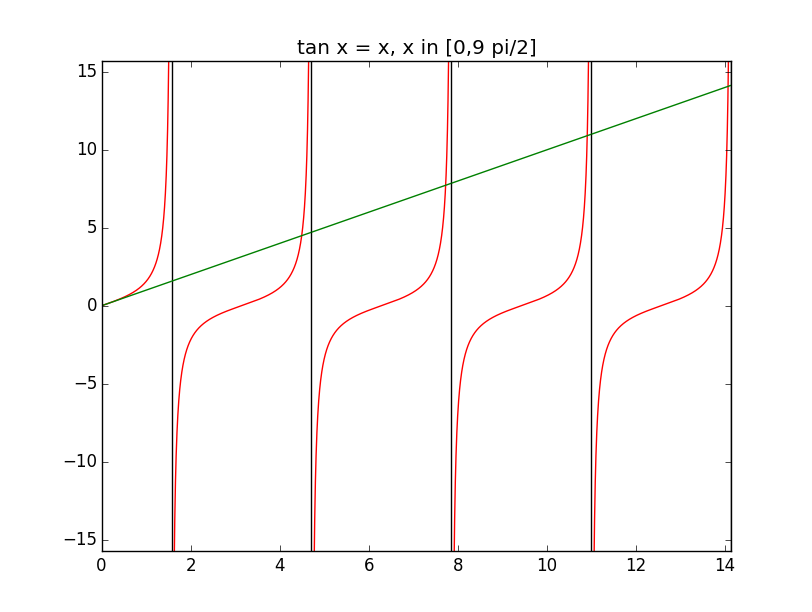
\includegraphics[scale=0.5]{tanxx.png}
 \caption{\emph{Solución gráfica de la ecuación tan x = x : son los puntos de intersección entre el gráfico dibujado con rojo y = tan x y el gráfico dibujado con verde y = x en el intervalo [0,9 pi/2]}}
\end{figure}

Como se ve también en el gráfico para $k R >0 \implies $ las soluciones se pueden aproximar $k R \approx \frac{(2n+1) \pi}{2} \implies k_n \approx \frac{(2n+1) \pi}{2 R}$

$\omega = c_s k \implies \omega_n \approx \sqrt{\frac{k_B}{m} T} \frac{(2n+1) \pi}{2 R}$


\paragraph 2

$I(\mu) = I_1 (\frac{2}{5} + \frac{3 \mu}{5}) $

\begin{figure}[!ht]
 \centering
 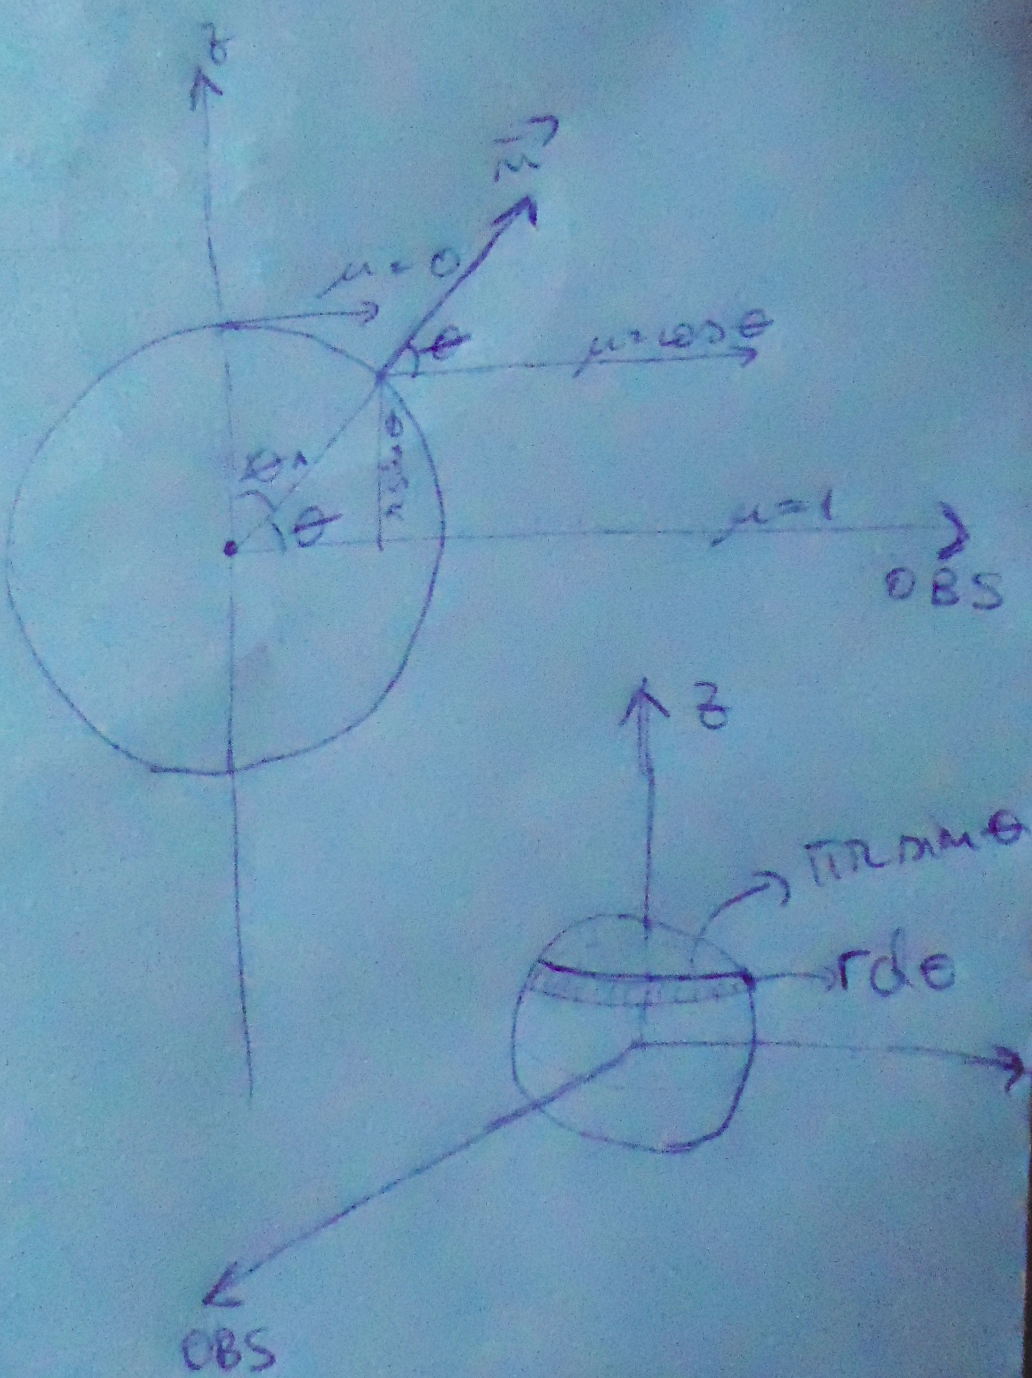
\includegraphics[scale=0.2]{p2s.png}
\end{figure}


Para encontrar la intensidad media sobre el disco 

hacemos la suposición que los rayos son paralelos a la línea de visión (hacía el observador) y que hacen el mismo ángulo $\theta$ 
como si estuvieran en el plano determinado por $\vec{e_z}$ y la línea de visión(independiente de $\phi$)

y luego integramos $I_{\nu} cos \theta$ sobre $dA = \pi r sin \theta r d\theta$ 
($I_{\nu}$ solo depende de $\theta$ con $\theta \in$ [-$\frac{\pi}{2}$, $\frac{\pi}{2}$] y
no depende de $\phi \in$ [-$\pi$, $\pi$]) y dividir por el area total (del disco)  

$I_m = 2 \int_{0}^{\frac{\pi}{2}} {r d\theta \pi r sin \theta I_{\nu}(\theta) cos \theta d\theta} \frac{1}{\pi r^2}$

(se puso el factor 2 enfrente y la integral entre 0 y $\frac{\pi}{2}$ porque $sin(\theta)$ es negativo entre -$\frac{\pi}{2}$ y 0 que corresponde
a la parte de abajo del disco con $z  <  0$ que tiene la misma distribución de intensidad que la parte de arriba)

Notando $\mu = cos \theta$

$I_m = 2 \int_{0}^{1} { I_{\nu}(\mu) \mu  d\mu} $

Reemplazando:

$I_{\nu}(\mu) = I_1 (\frac{2}{5} + \frac{\mu}{5}) $


$I_m = 2 I_1 \int_{0}^{1} (\frac{ 2\mu}{5} + \frac{ 3\mu^2}{5}) d\mu $

$I_m = 2 I_1 (\frac{ \mu^2}{5} + \frac{ \mu^3}{5} ) |_{0}^{1}$

$I_m = \frac{4 I_1}{5}$

Comprobación:

\begin{enumerate}

\item he commprobado algunos valores del gráfico de la hoja para ver si cumplen la relación

\item he escalado un gráfico aleatorio

\begin{figure}[!ht]
 \centering
 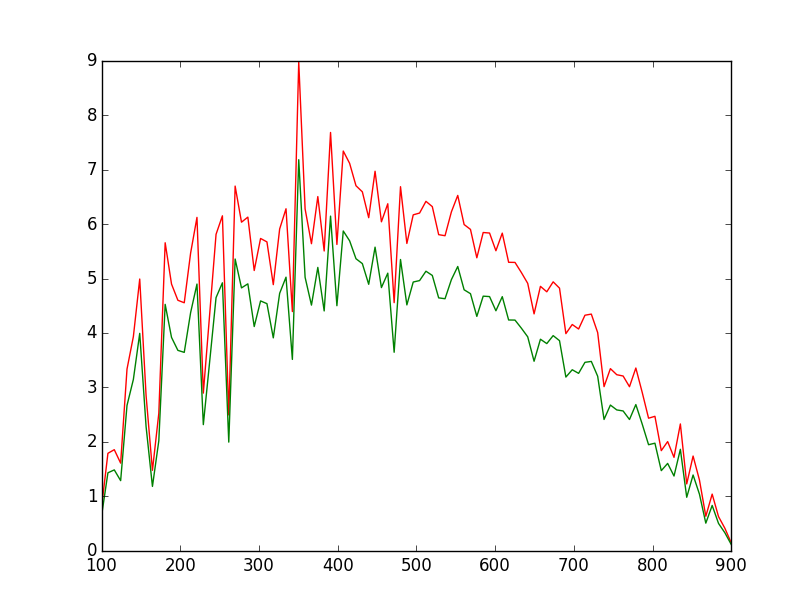
\includegraphics[scale=0.4]{ld.png}
 \caption{\emph{Intensidad al centro arriba (con rojo) - generada de forma más o menos aleatoria - la intensidad media - abajo (con verde)
que es el gráfico de arriba escalado con 4/5 - los gradientes también se escalan}}
\end{figure}

\end{enumerate}



\newpage


\paragraph 3

La temperatura efectiva de una  estrella con radio $R_{*}$ y luminosidad L es la temperatura de un cuerpo negro con la misma luminosidad

$L = F_{rad}(Teff)  4 \pi R_{*}^2$

$F_{rad}(T)$ es el flujo radiativo emitido por un cuerpo negro a temperatura T

Hay que encontrar el expresión para  $F_{rad}(T) $ empezando con la función de Planck 

\textbf{Definición del flujo radiativo}:

La intensidad $I_{\nu}$ se define como la energía de radiación  con frecuencia entre $\nu$ y $\nu + d\nu$ que pasa por el área dA 
en una dirección a un ángulo 
$\theta$ con respecto la normal al aŕea  en en ángulo sólido $d\omega$ y tiempo dt

$I_{\nu} = f(\vec{r}, cos \theta)$, $\vec{r} = (r, \theta, \phi)$ en coordenadas esféricas

$I_{\nu} = \frac{dE_{\nu}}{cos \theta dt d\nu d\omega dA} $


\begin{figure}[!ht]
 \centering
 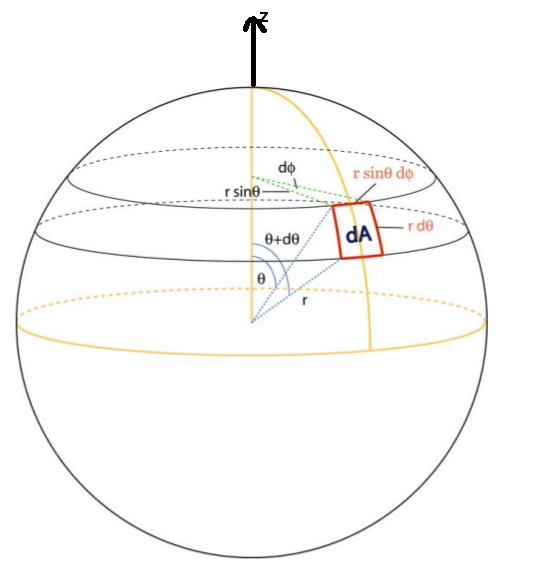
\includegraphics[scale=0.4]{sph.png}
 \caption{\emph{El angulo solido $d\omega$ subtendido por el área dA  \url{http://www.ifa.hawaii.edu/users/kud/teaching_09/3_Radiative_transfer.pdf}}}
\end{figure}


El flujo radiativo es la energía de radiación  con frecuencia entre $\nu$ y $\nu + d\nu$ que pasa por el área dA en el tiempo dt

Imaginando el centro de la esféra un punto P situado a radio R en la estrella , con la normal en la dirección $\vec{e_z}$

para determinar el flujo radiativo hay que tener en cuenta  las contribuciones de la intensidad en la esféra de radio r   

(hay que integrar $I_{\nu} cos \theta $ sobre el ángulo sólido $d\omega $ para $\theta \in$ [0, $\pi$] y $\phi \in $[0, 2$\pi$])

$dA = r^2 sin \theta d\theta d\phi $

$\frac{d\omega}{4\pi} = \frac{dA}{4 \pi r^2}  \implies d\omega = sin \theta d\theta d\phi$


$F_{\nu} = \int{I_{\nu}cos \theta d\omega} = \int_0^{2 \pi}{\int_{0}^{\pi}{I_{\nu} cos \theta sin \theta d\theta } d\phi }$

Suponiendo $I_{\nu}$ tiene  simetría acimutal (no depende del ángulo $\phi$):

$F_{\nu} = 2 \pi \int_0^{\pi}{I_{\nu}cos \theta sin \theta d\theta } $

Cambio de variable $cos \theta = \mu$

$F_{\nu} = 2 \pi \int_{-1}^{1}{I_{\nu} \mu d\mu } $

Notamos 

$F_{\nu}^{+} = 2 \pi \int_{0}^{1}{I_{\nu} \mu d\mu } $  (el flujo hacía afuera, $\theta \in$ [0, $\frac{\pi}{2}$]) 

$F_{\nu}^{-} = 2 \pi \int_{-1}^{0}{I_{\nu} \mu d\mu } $  (el flujo hacía adentro, $\theta \in$ [$-\frac{\pi}{2}$, 0])

El flujo total:

$F_{\nu} = F_{\nu}^{+} + F_{\nu}^{-}$

Suponemos la radiación isótropa ($I_{\nu}$ no depende de $\theta$)

$F_{\nu}^{+} = -F_{\nu}^{-} =   \pi I_{\nu} $

$F_{\nu} = 0$ 

Notamos el flujo radiativo  en la superficie de la estrella:

$F_{\nu}^{rad} = F_{\nu}^{+}(R_{*}) $ (en la superficie no hay flujo hacía adentro)


En el caso del cuerpo negro la intensidad es  \textbf{la función de Planck}:

$I_{\lambda} = B_{\lambda}(T) = \frac{2 h c^2}{\lambda ^5} \frac{1}{exp(\frac{h c}{\lambda k T}) -1 }$  

$F_{rad}(T) = \pi \int_{0}^{\infty} {B_{\lambda}(T) d{\lambda}} = \pi \int_{0}^{\infty} {B_{\nu}(T) d{\nu}} $

$F_{rad}(T) = \pi \int_{0}^{\infty} \frac{2 h \nu^3}{c^2} \frac{1}{exp(\frac{h \nu}{k T}) -1 } $

Cambio de variable $u = \frac{h \nu}{k T} \implies \nu = \frac{k T}{h} u$ y $ d\nu = \frac{k T}{h} du$

$F_{rad}(T) = \pi \frac{2 h}{c^2} (\frac{k T}{h})^4  \int_{0}^{\infty} \frac{u^3}{e^u - 1 }du $

$\int_{0}^{\infty} \frac{u^3}{e^u - 1 }du = \frac{\pi^4}{15} $ (de mathematica)

y notando $\sigma = \frac{2 \pi^5 k^4}{15 c^2 h^3}$

$F_{rad}(T) = \sigma  T^4 $ 

$ T_{eff} =  (\frac{L}  {4 \pi \sigma R_{*}^2})^{\frac{1}{4}}$

\paragraph 4

$\frac{\Delta \lambda_D} {\lambda_0}= \frac{\Delta \nu_D} {\nu_0} = \frac{v}{c} \implies$

$\Delta \lambda_D = \frac{\lambda_0}{c} \sqrt{\frac{k_B T}{m} + v_{mic}^2} $

Teniendo en cuenta que las líneas de FeI  se  forman a menos altura (15648A  a 20 km y T $\approx$  6000K y 6302A a 170 km y T $\approx$  
5000K) a la diferencia de la línea de $H\alpha$  que se forma 
en la parte mas alta y más caliente ($\approx$ 15000K) de la atmósfera, $v_{mic} \approx 1000m/s$
y $m = m_u A$ donde $m_u$ es la masa de un protón y A es la masa atómica (1 para H y 56 para Fe)
se  calcula el desplazamiento Doppler (para cada velocidad por separado para ver el efecto de cada una: térmica, microturbulencia y total)


\begin{verbatim}
Line: Halpha , Lambda (A): 6563.0, T = 15000.0(K), A = 1, m=1.6605e-27 kg
vterm=1.1168e+04 m/s, vtot = 1.1212e+04 m/s
dlTerm = 2.4431e-01 A, dlMic = 2.1877e-02 A, dlTot = 2.4529e-01 A

Line: FeI , Lambda (A): 6302.0, T = 5000.0(K), A = 56, m=9.2990e-26 kg
vterm=8.6160e+02 m/s, vtot = 1.3200e+03 m/s
dlTerm = 1.8099e-02 A, dlMic = 2.1007e-02 A, dlTot = 2.7729e-02 A

Line: FeI , Lambda (A): 15648.0, T = 6000.0(K), A = 56, m=9.2990e-26 kg
vterm=9.4384e+02 m/s, vtot = 1.3751e+03 m/s
dlTerm = 4.9231e-02 A, dlMic = 5.2160e-02 A, dlTot = 7.1724e-02 A
\end{verbatim}

Para las lineas de hierro el efecto Doppler debido a la microturbulencia es parecido al efecto Doppler
debido al movimiento térmico(desplazamientos parecidos) , pero en el caso de la línea de emision de hidrógeno
la alta temperatura hace que el efecto térmico domine el efecto  de la microturbulencia
 
https://github.com/beevageeva/fsol/







\end{document}
